% \documentclass[a4paper,10pt]{article}
% \usepackage[utf8]{inputenc}
% \usepackage{tikz}
% \usepackage{pgf}
% \usepackage{amsmath}
% \usepackage{textcomp}
% \usetikzlibrary{calc}
% 
% %opening
% \title{}
% \author{}
% 
% \begin{document}
% 
% \maketitle
% 
% \begin{abstract}
% 
% \end{abstract}
% 
% \section{Message Passing}
 \begin{figure}[scale=1.25]
 \centering
  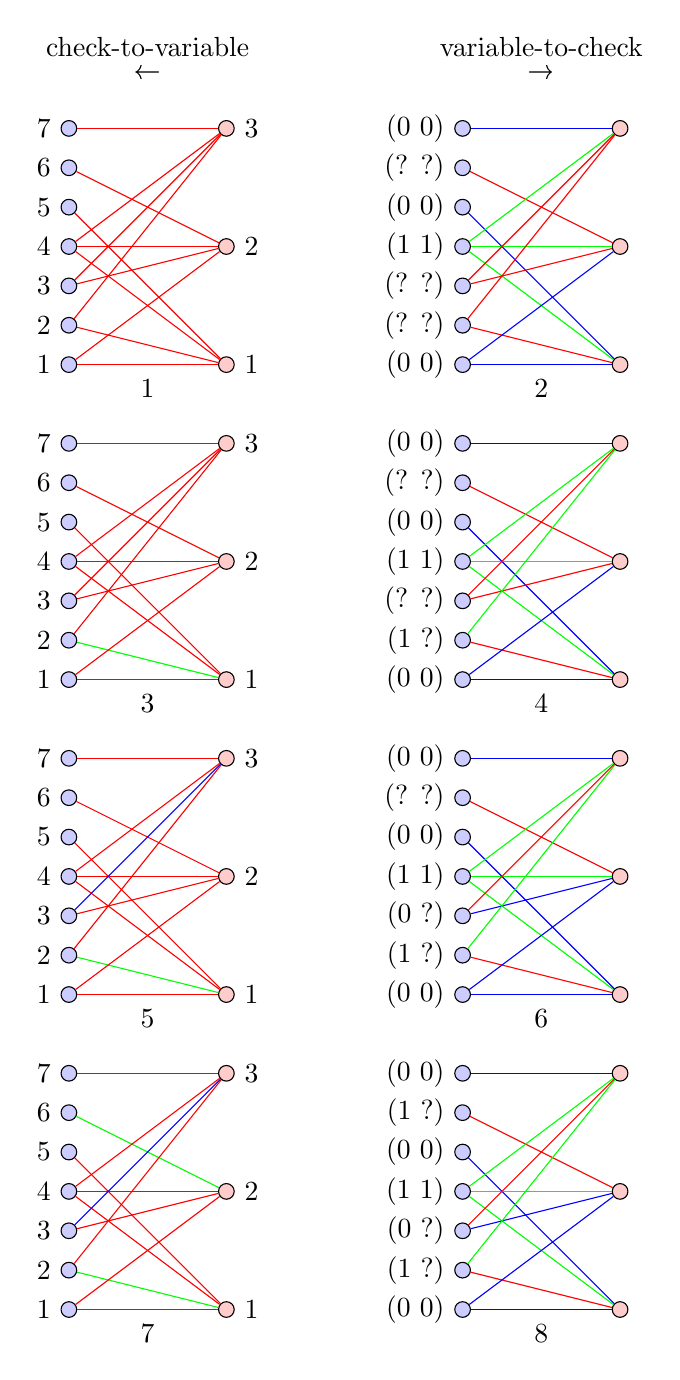
\begin{tikzpicture}
  \begin{scope}
    \begin{scope}
      \node[draw,circle,inner sep=2pt,fill=blue!20] (x7) at (0,0) [label=left:7] {};
      \node[draw,circle,inner sep=2pt,fill=blue!20] (x6) at (0,-0.5) [label=left:6] {};
      \node[draw,circle,inner sep=2pt,fill=blue!20] (x5) at (0,-1) [label=left:5] {};
      \node[draw,circle,inner sep=2pt,fill=blue!20] (x4) at (0,-1.5) [label=left:4] {};
      \node[draw,circle,inner sep=2pt,fill=blue!20] (x3) at (0,-2) [label=left:3] {};
      \node[draw,circle,inner sep=2pt,fill=blue!20] (x2) at (0,-2.5) [label=left:2] {};
      \node[draw,circle,inner sep=2pt,fill=blue!20] (x1) at (0,-3) [label=left:1] {};
      \node[draw,circle,inner sep=2pt,fill=red!20] (f3) at (2,0) [label=right:3] {};
      \node[draw,circle,inner sep=2pt,fill=red!20] (f2) at (2,-1.5) [label=right:2] {};
      \node[draw,circle,inner sep=2pt,fill=red!20] (f1) at (2,-3) [label=right:1] {};
      \draw[draw=red!100] (f1) ->  node [below = 2pt] {1} (x1);
      \draw[draw=red!100] (f1) ->  (x2);
      \draw[draw=red!100] (f1) ->  (x4);
      \draw[draw=red!100] (f1) ->  (x5);
      \draw[draw=red!100] (f2) ->  (x1);
      \draw[draw=red!100] (f2) ->  (x3);
      \draw[draw=red!100] (f2) ->  (x4);
      \draw[draw=red!100] (f2) ->  (x6);
      \draw[draw=red!100] (f3) ->  (x2);
      \draw[draw=red!100] (f3) ->  (x3);
      \draw[draw=red!100] (f3) ->  (x4);
      \draw[draw=red!100] (f3) -> node [above = 0.5cm] (larrow) {\textleftarrow} (x7);
      \node[above of=larrow, node distance=10pt] {check-to-variable};
    \end{scope}
    \begin{scope}[yshift=-4cm]
      \node[draw,circle,inner sep=2pt,fill=blue!20] (x7) at (0,0) [label=left:7] {};
      \node[draw,circle,inner sep=2pt,fill=blue!20] (x6) at (0,-0.5) [label=left:6] {};
      \node[draw,circle,inner sep=2pt,fill=blue!20] (x5) at (0,-1) [label=left:5] {};
      \node[draw,circle,inner sep=2pt,fill=blue!20] (x4) at (0,-1.5) [label=left:4] {};
      \node[draw,circle,inner sep=2pt,fill=blue!20] (x3) at (0,-2) [label=left:3] {};
      \node[draw,circle,inner sep=2pt,fill=blue!20] (x2) at (0,-2.5) [label=left:2] {};
      \node[draw,circle,inner sep=2pt,fill=blue!20] (x1) at (0,-3) [label=left:1] {};
      \node[draw,circle,inner sep=2pt,fill=red!20] (f3) at (2,0) [label=right:3] {};
      \node[draw,circle,inner sep=2pt,fill=red!20] (f2) at (2,-1.5) [label=right:2] {};
      \node[draw,circle,inner sep=2pt,fill=red!20] (f1) at (2,-3) [label=right:1] {};
      \draw[draw=red!100] (f1) ->  node [below = 2pt] {3} (x1);
      \draw[draw=green!100] (f1) ->  (x2);
      \draw[draw=red!100] (f1) ->  (x4);
      \draw[draw=red!100] (f1) ->  (x5);
      \draw[draw=red!100] (f2) ->  (x1);
      \draw[draw=red!100] (f2) ->  (x3);
      \draw[draw=red!100] (f2) ->  (x4);
      \draw[draw=red!100] (f2) ->  (x6);
      \draw[draw=red!100] (f3) ->  (x2);
      \draw[draw=red!100] (f3) ->  (x3);
      \draw[draw=red!100] (f3) ->  (x4);
      \draw[draw=red!100] (f3) ->  (x7);
    \end{scope}
    \begin{scope}[yshift=-8cm]
      \node[draw,circle,inner sep=2pt,fill=blue!20] (x7) at (0,0) [label=left:7] {};
      \node[draw,circle,inner sep=2pt,fill=blue!20] (x6) at (0,-0.5) [label=left:6] {};
      \node[draw,circle,inner sep=2pt,fill=blue!20] (x5) at (0,-1) [label=left:5] {};
      \node[draw,circle,inner sep=2pt,fill=blue!20] (x4) at (0,-1.5) [label=left:4] {};
      \node[draw,circle,inner sep=2pt,fill=blue!20] (x3) at (0,-2) [label=left:3] {};
      \node[draw,circle,inner sep=2pt,fill=blue!20] (x2) at (0,-2.5) [label=left:2] {};
      \node[draw,circle,inner sep=2pt,fill=blue!20] (x1) at (0,-3) [label=left:1] {};
      \node[draw,circle,inner sep=2pt,fill=red!20] (f3) at (2,0) [label=right:3] {};
      \node[draw,circle,inner sep=2pt,fill=red!20] (f2) at (2,-1.5) [label=right:2] {};
      \node[draw,circle,inner sep=2pt,fill=red!20] (f1) at (2,-3) [label=right:1] {};
      \draw[draw=red!100] (f1) ->  node [below = 2pt] {5} (x1);
      \draw[draw=green!100] (f1) ->  (x2);
      \draw[draw=red!100] (f1) ->  (x4);
      \draw[draw=red!100] (f1) ->  (x5);
      \draw[draw=red!100] (f2) ->  (x1);
      \draw[draw=red!100] (f2) ->  (x3);
      \draw[draw=red!100] (f2) ->  (x4);
      \draw[draw=red!100] (f2) ->  (x6);
      \draw[draw=red!100] (f3) ->  (x2);
      \draw[draw=blue!100] (f3) ->  (x3);
      \draw[draw=red!100] (f3) ->  (x4);
      \draw[draw=red!100] (f3) ->  (x7);
    \end{scope}
    \begin{scope}[yshift=-12cm]
      \node[draw,circle,inner sep=2pt,fill=blue!20] (x7) at (0,0) [label=left:7] {};
      \node[draw,circle,inner sep=2pt,fill=blue!20] (x6) at (0,-0.5) [label=left:6] {};
      \node[draw,circle,inner sep=2pt,fill=blue!20] (x5) at (0,-1) [label=left:5] {};
      \node[draw,circle,inner sep=2pt,fill=blue!20] (x4) at (0,-1.5) [label=left:4] {};
      \node[draw,circle,inner sep=2pt,fill=blue!20] (x3) at (0,-2) [label=left:3] {};
      \node[draw,circle,inner sep=2pt,fill=blue!20] (x2) at (0,-2.5) [label=left:2] {};
      \node[draw,circle,inner sep=2pt,fill=blue!20] (x1) at (0,-3) [label=left:1] {};
      \node[draw,circle,inner sep=2pt,fill=red!20] (f3) at (2,0) [label=right:3] {};
      \node[draw,circle,inner sep=2pt,fill=red!20] (f2) at (2,-1.5) [label=right:2] {};
      \node[draw,circle,inner sep=2pt,fill=red!20] (f1) at (2,-3) [label=right:1] {};
      \draw[draw=red!100] (f1) ->  node [below = 2pt] {7} (x1);
      \draw[draw=green!100] (f1) ->  (x2);
      \draw[draw=red!100] (f1) ->  (x4);
      \draw[draw=red!100] (f1) ->  (x5);
      \draw[draw=red!100] (f2) ->  (x1);
      \draw[draw=red!100] (f2) ->  (x3);
      \draw[draw=red!100] (f2) ->  (x4);
      \draw[draw=green!100] (f2) ->  (x6);
      \draw[draw=red!100] (f3) ->  (x2);
      \draw[draw=blue!100] (f3) ->  (x3);
      \draw[draw=red!100] (f3) ->  (x4);
      \draw[draw=red!100] (f3) ->  (x7);
    \end{scope}
  \end{scope}
%=========================================================================================
  \begin{scope}[xshift=5cm]
    \begin{scope}
      \node[draw,circle,inner sep=2pt,fill=blue!20] (x7) at (0,0) [label=left:(0 0)] {};
      \node[draw,circle,inner sep=2pt,fill=blue!20] (x6) at (0,-0.5) [label=left:(? ?)] {};
      \node[draw,circle,inner sep=2pt,fill=blue!20] (x5) at (0,-1) [label=left:(0 0)] {};
      \node[draw,circle,inner sep=2pt,fill=blue!20] (x4) at (0,-1.5) [label=left:(1 1)] {};
      \node[draw,circle,inner sep=2pt,fill=blue!20] (x3) at (0,-2) [label=left:(? ?)] {};
      \node[draw,circle,inner sep=2pt,fill=blue!20] (x2) at (0,-2.5) [label=left:(? ?)] {};
      \node[draw,circle,inner sep=2pt,fill=blue!20] (x1) at (0,-3) [label=left:(0 0)] {};
      \node[draw,circle,inner sep=2pt,fill=red!20] (f3) at (2,0) {};
      \node[draw,circle,inner sep=2pt,fill=red!20] (f2) at (2,-1.5) {};
      \node[draw,circle,inner sep=2pt,fill=red!20] (f1) at (2,-3) {};
      \draw[draw=blue!100] (f1) ->  node [below = 2pt] {2} (x1);
      \draw[draw=red!100] (f1) ->  (x2);
      \draw[draw=green!100] (f1) ->  (x4);
      \draw[draw=blue!100] (f1) ->  (x5);
      \draw[draw=blue!100] (f2) ->  (x1);
      \draw[draw=red!100] (f2) ->  (x3);
      \draw[draw=green!100] (f2) ->  (x4);
      \draw[draw=red!100] (f2) ->  (x6);
      \draw[draw=red!100] (f3) ->  (x2);
      \draw[draw=red!100] (f3) ->  (x3);
      \draw[draw=green!100] (f3) ->  (x4);
      \draw[draw=blue!100] (f3) -> node [above = 0.5cm] (rarrow) {\textrightarrow} (x7);
      \node[above of=rarrow, node distance=10pt] {variable-to-check};
    \end{scope}
    \begin{scope}[yshift=-4cm]
      \node[draw,circle,inner sep=2pt,fill=blue!20] (x7) at (0,0) [label=left:(0 0)] {};
      \node[draw,circle,inner sep=2pt,fill=blue!20] (x6) at (0,-0.5) [label=left:(? ?)] {};
      \node[draw,circle,inner sep=2pt,fill=blue!20] (x5) at (0,-1) [label=left:(0 0)] {};
      \node[draw,circle,inner sep=2pt,fill=blue!20] (x4) at (0,-1.5) [label=left:(1 1)] {};
      \node[draw,circle,inner sep=2pt,fill=blue!20] (x3) at (0,-2) [label=left:(? ?)] {};
      \node[draw,circle,inner sep=2pt,fill=blue!20] (x2) at (0,-2.5) [label=left:(1 ?)] {};
      \node[draw,circle,inner sep=2pt,fill=blue!20] (x1) at (0,-3) [label=left:(0 0)] {};
      \node[draw,circle,inner sep=2pt,fill=red!20] (f3) at (2,0) {};
      \node[draw,circle,inner sep=2pt,fill=red!20] (f2) at (2,-1.5) {};
      \node[draw,circle,inner sep=2pt,fill=red!20] (f1) at (2,-3) {};
      \draw[draw=blue!100] (f1) ->  node [below = 2pt] {4} (x1);
      \draw[draw=red!100] (f1) ->  (x2);
      \draw[draw=green!100] (f1) ->  (x4);
      \draw[draw=blue!100] (f1) ->  (x5);
      \draw[draw=blue!100] (f2) ->  (x1);
      \draw[draw=red!100] (f2) ->  (x3);
      \draw[draw=green!100] (f2) ->  (x4);
      \draw[draw=red!100] (f2) ->  (x6);
      \draw[draw=green!100] (f3) ->  (x2);
      \draw[draw=red!100] (f3) ->  (x3);
      \draw[draw=green!100] (f3) ->  (x4);
      \draw[draw=blue!100] (f3) ->  (x7);
    \end{scope}
    \begin{scope}[yshift=-8cm]
      \node[draw,circle,inner sep=2pt,fill=blue!20] (x7) at (0,0) [label=left:(0 0)] {};
      \node[draw,circle,inner sep=2pt,fill=blue!20] (x6) at (0,-0.5) [label=left:(? ?)] {};
      \node[draw,circle,inner sep=2pt,fill=blue!20] (x5) at (0,-1) [label=left:(0 0)] {};
      \node[draw,circle,inner sep=2pt,fill=blue!20] (x4) at (0,-1.5) [label=left:(1 1)] {};
      \node[draw,circle,inner sep=2pt,fill=blue!20] (x3) at (0,-2) [label=left:(0 ?)] {};
      \node[draw,circle,inner sep=2pt,fill=blue!20] (x2) at (0,-2.5) [label=left:(1 ?)] {};
      \node[draw,circle,inner sep=2pt,fill=blue!20] (x1) at (0,-3) [label=left:(0 0)] {};
      \node[draw,circle,inner sep=2pt,fill=red!20] (f3) at (2,0) {};
      \node[draw,circle,inner sep=2pt,fill=red!20] (f2) at (2,-1.5) {};
      \node[draw,circle,inner sep=2pt,fill=red!20] (f1) at (2,-3) {};
      \draw[draw=blue!100] (f1) ->  node [below = 2pt] {6} (x1);
      \draw[draw=red!100] (f1) ->  (x2);
      \draw[draw=green!100] (f1) ->  (x4);
      \draw[draw=blue!100] (f1) ->  (x5);
      \draw[draw=blue!100] (f2) ->  (x1);
      \draw[draw=blue!100] (f2) ->  (x3);
      \draw[draw=green!100] (f2) ->  (x4);
      \draw[draw=red!100] (f2) ->  (x6);
      \draw[draw=green!100] (f3) ->  (x2);
      \draw[draw=red!100] (f3) ->  (x3);
      \draw[draw=green!100] (f3) ->  (x4);
      \draw[draw=blue!100] (f3) ->  (x7);
    \end{scope}
    \begin{scope}[yshift=-12cm]
      \node[draw,circle,inner sep=2pt,fill=blue!20] (x7) at (0,0) [label=left:(0 0)] {};
      \node[draw,circle,inner sep=2pt,fill=blue!20] (x6) at (0,-0.5) [label=left:(1 ?)] {};
      \node[draw,circle,inner sep=2pt,fill=blue!20] (x5) at (0,-1) [label=left:(0 0)] {};
      \node[draw,circle,inner sep=2pt,fill=blue!20] (x4) at (0,-1.5) [label=left:(1 1)] {};
      \node[draw,circle,inner sep=2pt,fill=blue!20] (x3) at (0,-2) [label=left:(0 ?)] {};
      \node[draw,circle,inner sep=2pt,fill=blue!20] (x2) at (0,-2.5) [label=left:(1 ?)] {};
      \node[draw,circle,inner sep=2pt,fill=blue!20] (x1) at (0,-3) [label=left:(0 0)] {};
      \node[draw,circle,inner sep=2pt,fill=red!20] (f3) at (2,0) {};
      \node[draw,circle,inner sep=2pt,fill=red!20] (f2) at (2,-1.5) {};
      \node[draw,circle,inner sep=2pt,fill=red!20] (f1) at (2,-3) {};
      \draw[draw=blue!100] (f1) ->  node [below = 2pt] {8} (x1);
      \draw[draw=red!100] (f1) ->  (x2);
      \draw[draw=green!100] (f1) ->  (x4);
      \draw[draw=blue!100] (f1) ->  (x5);
      \draw[draw=blue!100] (f2) ->  (x1);
      \draw[draw=blue!100] (f2) ->  (x3);
      \draw[draw=green!100] (f2) ->  (x4);
      \draw[draw=red!100] (f2) ->  (x6);
      \draw[draw=green!100] (f3) ->  (x2);
      \draw[draw=red!100] (f3) ->  (x3);
      \draw[draw=green!100] (f3) ->  (x4);
      \draw[draw=blue!100] (f3) ->  (x7);
    \end{scope}
  \end{scope}
  \end{tikzpicture}
\caption{Message-passing decoding of the [7, 4, 3] Hamming code with the received code word y = (0, ?, ?, 1, 0, ?, 0).
The left column is represents message passing from check to variable nodes. Right column represents message passing
from variable to check nodes. Red links represents erasure messages, blue links represents messages 1 (corresponds to codebit 0)
and green links represents message -1 (corresponds to codebit 1). The labels on the variable nodes in the right column represents
the pair (estimated bit, received bit)}
\label{fig:message_passing}
\end{figure}
% \end{document}